%! TEX root = main.tex  %
\documentclass[main.tex]{subfiles} % Wichtig!

\begin{document}

\subsection{Storyboard BA-thesis-video}
Die erste Skizze auf Abbildung \ref{fig:storyboard} zeigt eine Küchenszene, in der jemand beginnt 
zu kochen. Sie zeigt ein Tablet als Kochhilfe und die Interaktion mit einem Sprachassistenten. 
Der erste Teil des Videos zeigt die Hands-free-Nutzung eines Sprachassistenten beim Kochen. 
Der Rest des Videos präsentiert die Bachelorarbeit 'Integration von Sprachsteuerung in mobilen Apps' 
als Slideshow. Das Storyboard besteht aus zwei Teilen: Einem Teaser-Clip mit Kochszene und einer 
anschliessenden Slideshow der BA.

\begin{figure}[H]
    \centering
    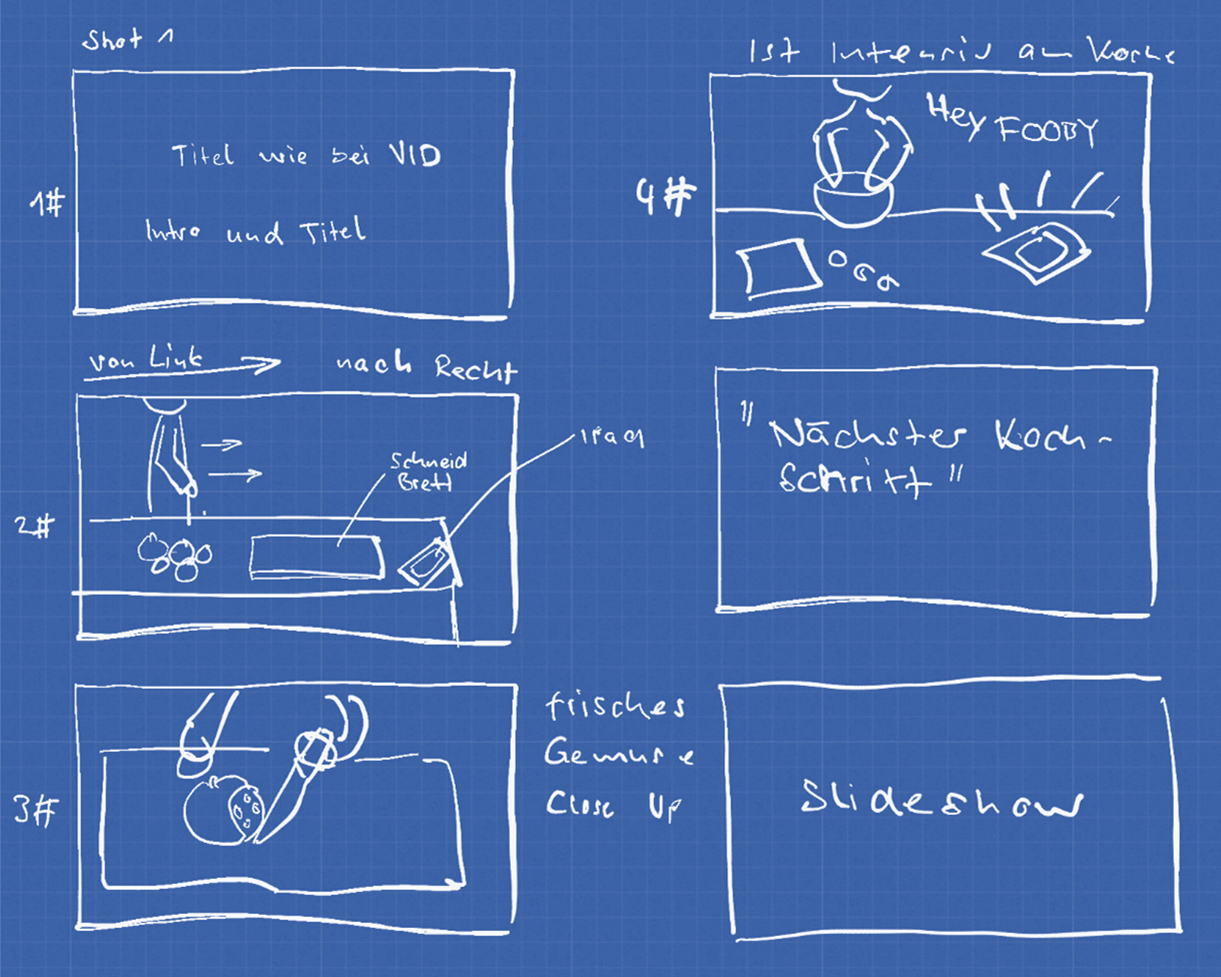
\includegraphics[width=0.85\textwidth]{img/storyboard-draft.png}
    \caption{Storyboard BA-thesis-video (Entwurf)}
    \label{fig:storyboard-draft}
\end{figure}

\noindent \newline
Die Skizze wurde in einem zweiten Schritt in ein Storyboard überführt. Das Storyboard ist in 
Abbildung \ref{fig:storyboard} zu sehen. Es zeigt die einzelnen Szenen des Videos.

\begin{figure}[H]
    \centering
    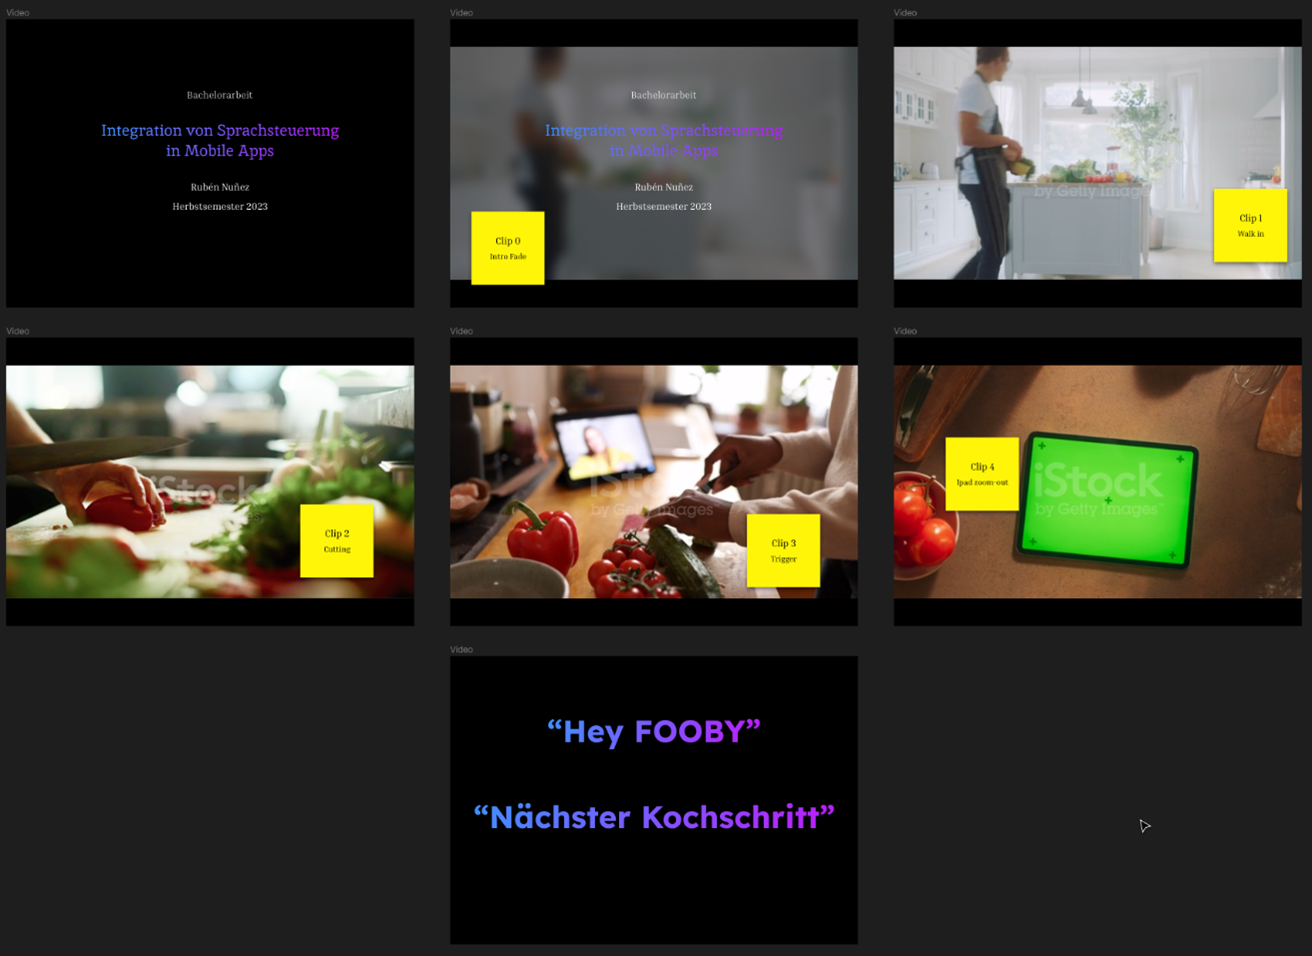
\includegraphics[width=0.85\textwidth]{img/storyboard.png}
    \caption{Storyboard BA-thesis-video}
    \label{fig:storyboard}
\end{figure}

\noindent \newline
Erst wird der Titel der Bachelorarbeit gezeigt 1, wobei Fade-Transitions für einen 
übersichtlichen Übergang sorgen. In der ersten Videoszene 2 läuft jemand in die Küche, ohne 
dass das Gesicht gezeigt wird. Die Ka-mera bewegt sich in die entgegengesetzte Richtung, um die 
Laufrichtung zu betonen. Die Szene dau-ert maximal 3 Sekunden. Szene 3 zeigt eine Nahaufnahme vom 
Gemüseschneiden, um das Kochen zu betonen und eine schöne Kulisse zu schaffen. Diese Szene dauert 
maximal 2-3 Sekunden.In Szene 4 sagt der Protagonist 'Hey FOOBY', während das Tablet im Blickfeld 
ist und visuelles oder akustisches Feedback gibt. Danach folgt der Befehl 'Nächster Kochschritt'. 
Die letzte Szene 5 zeigt das Tablet von oben, mit den Kochschritten und der Ausführung des 
Befehls. Dann folgt die Slideshow, die eine Kurzfassung der Endpräsentation enthält. Diese 
beschreibt die erarbeitete Bachelorarbeit, insbesondere im Hinblick auf die Lösung.


\end{document}
